\subsection{Kempe-chains}

Drawing again inspiration from the proof of the five color theorem. We had essentially proven that the vertex with five neighbors is a 0-reducible configuration. The key weapon we used in this proof was the notion of \textit{chains}. Therefore, we will try using them to prove general $k$-reducibility as well by giving a proper definition.

\begin{definition}
    Let $G_{ab}(x)$ be the subgraph consisting of all the vertices colored $ab$ in the coloring $x$ of $G$.
    Then the \emph{Kempe-chain} $\kappa_{ab}(v)$ or \emph{$ab$-chain} of the vertex $v$ is the component of $G_{ab}(x)$ that contains $v$. 
\end{definition}

\begin{figure}[!ht]
    \centering
    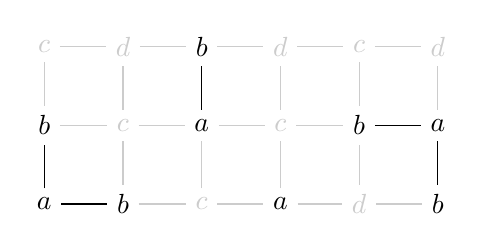
\begin{tikzpicture}[scale=1]
        \node (x11) at (0, 0) { $a$ };
        \node (x12) at (1, 0) { $b$ };
        \node[opacity=0.2] (x13) at (2, 0) { $c$ };
        \node (x21) at (0, 1) { $b$ };
        \node[opacity=0.2] (x22) at (1, 1) { $c$ };
        \node (x23) at (2, 1) { $a$ };
        \node[opacity=0.2] (x31) at (0, 2) { $c$ };
        \node[opacity=0.2] (x32) at (1, 2) { $d$ };
        \node (x33) at (2, 2) { $b$ };
        \node (y11) at (3, 0) { $a$ };
        \node[opacity=0.2] (y12) at (4, 0) { $d$ };
        \node (y13) at (5, 0) { $b$ };
        \node[opacity=0.2] (y21) at (3, 1) { $c$ };
        \node (y22) at (4, 1) { $b$ };
        \node (y23) at (5, 1) { $a$ };
        \node[opacity=0.2] (y31) at (3, 2) { $d$ };
        \node[opacity=0.2] (y32) at (4, 2) { $c$ };
        \node[opacity=0.2] (y33) at (5, 2) { $d$ };

        \draw (x11) -- (x12);
        \draw[opacity=0.2] (x12) -- (x13);

        \draw[opacity=0.2] (x21) -- (x22);
        \draw[opacity=0.2] (x22) -- (x23);
        \draw[opacity=0.2] (x31) -- (x32);
        \draw[opacity=0.2] (x32) -- (x33);

        \draw (x11) -- (x21);
        \draw[opacity=0.2] (x21) -- (x31);
        \draw[opacity=0.2] (x12) -- (x22) -- (x32);
        \draw[opacity=0.2] (x13) -- (x23);
        \draw (x23) -- (x33);

        \draw[opacity=0.2] (y11) -- (y12) -- (y13);
        \draw[opacity=0.2] (y21) -- (y22);
        \draw (y22) -- (y23);
        \draw[opacity=0.2] (y31) -- (y32) -- (y33);

        \draw[opacity=0.2] (y11) -- (y21) -- (y31);
        \draw[opacity=0.2] (y12) -- (y22) -- (y32);
        \draw (y13) -- (y23);
        \draw[opacity=0.2] (y23) -- (y33);

        \draw[opacity=0.2] (x13) -- (y11);
        \draw[opacity=0.2] (x23) -- (y21);
        \draw[opacity=0.2] (x33) -- (y31);
    \end{tikzpicture}
    \caption{The components of $G_{ab}(x)$ for a planar graph $G$ and its coloring $x$ are highlighted. We write $\chain{u}{v}{ab}$ or $u \in \kappa_{ab}(v)$ if $u$ and $v$ are on the same component.}
    \label{fig:kempetut}
\end{figure}

As we have seen before, we can flip the colors of a chain $\kappa_{ab}(v)$ without breaking the current coloring. Imagine in your head how you can swap the chains in Figure \ref{fig:kempetut} for example. This key property of chains will allow us to obtain new ring colorings.

Judging only from the colors of a ring such as in $abcab$, we have no information on the chains that are present. This information is important because two vertices of the ring that belong to the same chain must be flipped together.

To include this information in a ring coloring, Birkhoff devised the notion of a \textit{scheme}. He simply draws a line between two colors on the ring if they belong to the same Kempe-chain.

\begin{definition}
    Given a coloring $x$ of a planar graph $G$ and the colors on its ring $x(R)$. The \emph{scheme} on $R$ of $x$ consists of $x(R)$ with knowledge whether $u \in \kappa_{ab}(v)$ for two ring vertices $u,v \in R$ and colors $ab$.
\end{definition}
\begin{figure}[!ht]
    \centering
    \begin{tikzpicture}[scale=1.0, mid arrow/.style={
        postaction={ decorate, decoration={ markings, mark=at position 0.6 with { \arrow[black]{>>} } } } }]

        \node[circle, fill, scale=0.015cm, opacity=0.2] (v) at (0, 0) { };
        \node[circle, fill, scale=0.015cm, label=above:$a$] (l1) at (0, 1) { };
        \node[circle, fill, scale=0.015cm, label=right:$b$] (l2) at (0.9, 0.30) { };
        \node[circle, fill, scale=0.015cm, label=below:$c$] (l3) at (0.6, -0.77) {};
        \node[circle, fill, scale=0.015cm, label=below:$a$] (l4) at (-0.6, -0.77) {};
        \node[circle, fill, scale=0.015cm, label=left:$b$] (l5) at (-0.9, 0.30) {};
        \node[circle, fill, scale=0.015cm, label=above:$c$] (c1) at (0.7, 1) {};
        \node[circle, fill, scale=0.015cm, label=right:$a$] (c2) at (1.32, 0.68) {};
        \node[circle, fill, scale=0.015cm, label=right:$c$] (c3) at (1.45, 0.05) {};
        \node[circle, fill, scale=0.015cm, label=right:$a$] (c4) at (1.1, -0.49) {};
        \draw[mid arrow] (l1) -- (l2);
        \draw (l2) -- (l3) -- (l4) -- (l5) -- (l1);
        \draw (l1) -- (c1) -- (c2) -- (c3) -- (c4) -- (l3);
        \draw[opacity=0.2] (l1) -- (v);
        \draw[opacity=0.2] (l2) -- (v);
        \draw[opacity=0.2] (l3) -- (v);
        \draw[opacity=0.2] (l4) -- (v); 
        \draw[opacity=0.2] (l5) -- (v);
        \node (impl) at (3, 0) { $\hspace{1cm} \implies \hspace{0.3cm} \begin{matrix}
            \scheme{a,b,c,a,b}{ 13a } \\
            \scheme{a,b,c,a,b}{ 25d- }
        \end{matrix}$ };
        
    \end{tikzpicture}
    \caption{Two ring schemes that are derived from a graph coloring. We only consider the chains on one side of the ring. The strikethrough $\cancel{d}$ indicates absence of a chain. Refer to the main.tex file \cite{github} for the \;\LaTeX\; source of this notation. }
    \label{fig:schemes}
\end{figure}

A coloring can be treated as a scheme without information on chains. A scheme can be treated as a coloring. As such, we will use them interchangeably from now on. 

Given the information of Kempe-chains on a coloring, we can start modifying the colors of the ring by flipping chains. We call any coloring that can be derived in this manner an \textit{implied coloring} of the scheme. 

\begin{definition}
    Given two schemes $x$ and $y$. We say that $x$ implies $y$ if $x=y$ or $y$ can be obtained from $x$ by flipping a Kempe-chain. Write $x\compat y$.
\end{definition}

For example, the two schemes from Figure \ref{fig:schemes} have the following implications (change is highlighted).

\begin{equation*}
    \scheme{a,b,c,a,b}{ 13a } \compat \scheme{a,b,c,a,\textbf{d}}{{13a}}, \quad \quad
    \scheme{a,b,c,a,b}{ 25d- } \compat \scheme{a,\textbf{d},c,a,b}{{25d-}}.
\end{equation*}

We have now built a strong theory to modify ring colorings using schemes and Kempe-chains, all inspired by the proof of the five color theorem. You can try for yourself to rewrite that proof using scheme notation (assume that the neighbors form a ring). With these tools, we are now ready to prove the $k$-reducibility of rings.